% 2007 年上海卷文科第 16 题：正四棱锥 P-ABCD。
% 方形底面按斜投影示意；后侧底棱 CD、AD 及棱 PD 以虚线表示。
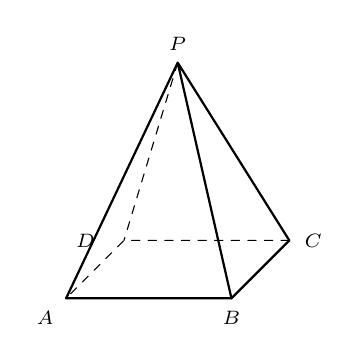
\begin{tikzpicture}[x=1.05cm,y=1.05cm,line cap=round,line join=round,
  every node/.style={font=\scriptsize}]
  \coordinate (A) at (0,0);
  \coordinate (B) at (2,0);
  \coordinate (C) at (2.7,.7);
  \coordinate (D) at (.7,.7);
  \coordinate (P) at (1.35,2.85);

  \draw[thick] (A)--(B)--(C);
  \draw[dashed] (C)--(D)--(A);
  \draw[thick] (P)--(A) (P)--(B) (P)--(C);
  \draw[dashed] (P)--(D);

  \node[below left=1pt] at (A) {$A$};
  \node[below=1pt] at (B) {$B$};
  \node[right=2pt] at (C) {$C$};
  \node[left=7pt] at (D) {$D$};
  \node[above=1pt] at (P) {$P$};
\end{tikzpicture}
